%%%%%%%%%%%%%%%%%%%%%%%%%%%%%%%%%%%%%%%%%%%%%%%%%%%%%%%%%%%%%%%%%%%%%%%%%%%%%%%%%%
\begin{frame}[fragile]\frametitle{}

\begin{center}
{\Large PoS in NLTK}
\end{center}
\end{frame}

%%%%%%%%%%%%%%%%%%%%%%%%%%%%%%%%%%%%%%%%%%%%%%%%%%%%%%%%%%%%%%%%%%%%%%%%%%%%%%%%%%
\begin{frame}[fragile]\frametitle{POS-tagger}
Processes a sequence of words, and attaches a part of speech tag to each word:
\begin{lstlisting}
import nltk
text = nltk.word_tokenize("And now for something completely different")
nltk.pos_tag(text)
\end{lstlisting}
 Output:
\begin{lstlisting}
[('And', 'CC'),
 ('now', 'RB'),
 ('for', 'IN'),
 ('something', 'NN'),
 ('completely', 'RB'),
 ('different', 'JJ')]
\end{lstlisting}
\end{frame}

%%%%%%%%%%%%%%%%%%%%%%%%%%%%%%%%%%%%%%%%%%%%%%%%%%%%%%%%%%%%%%%%%%%%%%%%%%%%%%%%%%
\begin{frame}[fragile]\frametitle{Impo PoS tags}

\begin{center}
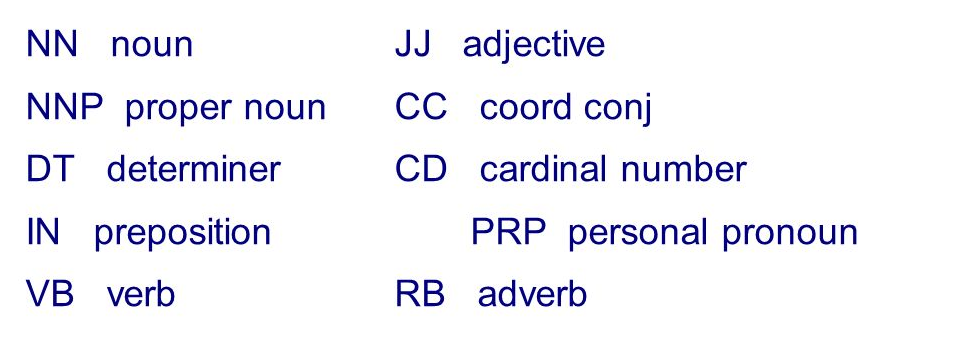
\includegraphics[width=\linewidth,keepaspectratio]{treepos}
\end{center}
  (Ref: Penn Treebank)
\end{frame}

%%%%%%%%%%%%%%%%%%%%%%%%%%%%%%%%%%%%%%%%%%%%%%%%%%%%%%%%%%%%%%%%%%%%%%%%%%%%%%%%%%
\begin{frame}[fragile]\frametitle{Verb Tags}

\begin{center}
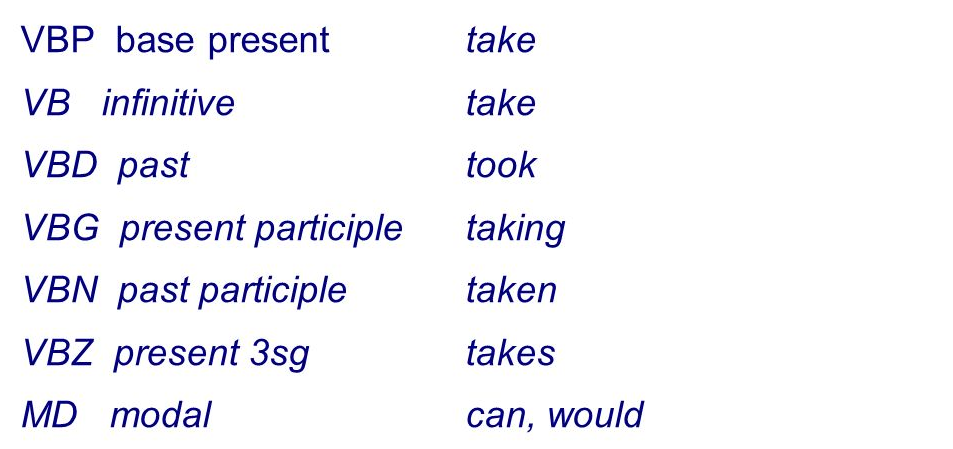
\includegraphics[width=\linewidth,keepaspectratio]{treevbpos}
\end{center}
  (Ref: Penn Treebank)
\end{frame}

%%%%%%%%%%%%%%%%%%%%%%%%%%%%%%%%%%%%%%%%%%%%%%%%%%%%%%%%%%%%%%%%%%%%%%%%%%%%%%%%%%
\begin{frame}[fragile]\frametitle{POS-tagger}
NLTK provides documentation for each tag, which can be queried using the tag, e.g. \lstinline| nltk.help.upenn_tagset('RB')|, or a regular expression, e.g. \lstinline|nltk.help.upenn_tagset('NN.*')|.
\begin{lstlisting}
nltk.help.upenn_tagset('RB')
\end{lstlisting}
 Output:
\begin{lstlisting}
RB: adverb
    occasionally unabatingly maddeningly adventurously professedly
    stirringly prominently technologically magisterially predominately
    swiftly fiscally pitilessly ...
\end{lstlisting}
\end{frame}

%
%%%%%%%%%%%%%%%%%%%%%%%%%%%%%%%%%%%%%%%%%%%%%%%%%%%%%%%%%%%%%%%%%%%%%%%%%%%%%%%%%%%
%\begin{frame}[fragile]\frametitle{POS-tagger with homonyms}
%
%\begin{lstlisting}
%text = nltk.word_tokenize("They refuse to permit us to obtain the refuse permit")
%nltk.pos_tag(text)
%\end{lstlisting}
% Output:
%\begin{lstlisting}
%[('They', 'PRP'),
% ('refuse', 'VBP'),
% ('to', 'TO'),
% ('permit', 'VB'),
% ('us', 'PRP'),
% ('to', 'TO'),
% ('obtain', 'VB'),
% ('the', 'DT'),
% ('refuse', 'NN'),
% ('permit', 'NN')]
%\end{lstlisting}
%refUSE is a verb meaning "deny," while REFuse is a noun meaning "trash". We need to know which word is being used in order to pronounce the text correctly.
%\end{frame}
%
%%%%%%%%%%%%%%%%%%%%%%%%%%%%%%%%%%%%%%%%%%%%%%%%%%%%%%%%%%%%%%%%%%%%%%%%%%%%%%%%%%%
%\begin{frame}[fragile]\frametitle{POS-tagger with Wordnet}
%
%\begin{lstlisting}
%from nltk.corpus import wordnet as wn
%wn.synsets('refuse')
%senses = [(s.lemma_names(), s.definition(), s.examples()) for s in wn.synsets('refuse')]
%for s in senses:
%    print "Lemma name:", s[0]
%    print "Definition:", s[1]
%    print "Examples  :", s[2]
%    print "======================="
%\end{lstlisting}
% Output:
%\begin{lstlisting}
%[Synset('garbage.n.01'),
% Synset('refuse.v.01'),
% Synset('refuse.v.02'),
% Synset('defy.v.02'),
% Synset('deny.v.04'),
% Synset('resist.v.05'),
% Synset('reject.v.06')]
%Lemma name: [u'garbage', u'refuse', u'food_waste', u'scraps']
%Definition: food that is discarded (as from a kitchen)
%Examples  : []
%=======================
%Lemma name: [u'refuse', u'decline']
%Definition: show unwillingness towards
%Examples  : [u'he declined to join the group on a hike']
%\end{lstlisting}
%\end{frame}


%%%%%%%%%%%%%%%%%%%%%%%%%%%%%%%%%%%%%%%%%%%%%%%%%%%%%%%%%%%%%%%%%%%%%%%%%%%%%%%%%%
\begin{frame}[fragile]\frametitle{Tagging in NLTK}
\textcolor{black}{The simplest possible tagger tags everything as a noun:}
\small
\begin{lstlisting}
text = `There are 11 players in a football team'
text_tokens = text.split()
# ['There', 'are', '11', 'players', 'in', 'a', 'football', 'team']
\end{lstlisting}
  
\begin{lstlisting}
import nltk
mytagger = nltk.DefaultTagger('NN')
for t in mytagger.tag(text_tokens):
    print t
# ('There', 'NN')
# ('are', 'NN')
# ...
\end{lstlisting}
\end{frame}
%
%%%%%%%%%%%%%%%%%%%%%%%%%%%%%%%%%%%%%%%%%%%%%%%%%%%%%%%%%%%%%%%%%%%%%%%%%%%%%%%%%%%
%\begin{frame}[fragile]\frametitle{Part-of-Speech Ambiguity}
%
%\begin{center}
%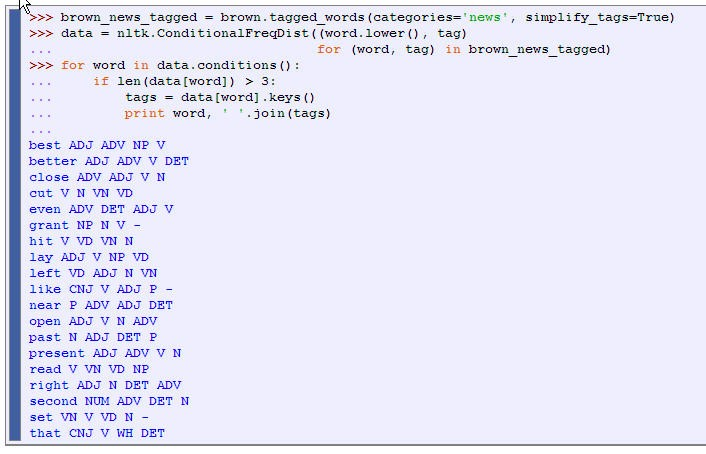
\includegraphics[width=\linewidth,keepaspectratio]{pos2}
%\end{center}
%  
%\end{frame}


%%%%%%%%%%%%%%%%%%%%%%%%%%%%%%%%%%%%%%%%%%%%%%%%%%%%%%%%%%%%%%%%%%%%%%%%%%%%%%%%%%
\begin{frame}[fragile]\frametitle{A regular expression tagger}
\textcolor{black}{
The regular expression tagger assigns tags to tokens on the basis of matching patterns. For instance, we might guess that any word ending in ed is the past participle of a verb, and any word ending with 's is a possessive noun. We can express these as a list of regular expressions:}
\small
\begin{lstlisting}
>>> patterns = [
...     (r'.*ing$', 'VBG'),               # gerunds
...     (r'.*ed$', 'VBD'),                # simple past
...     (r'.*es$', 'VBZ'),                # 3rd singular present
...     (r'.*ould$', 'MD'),               # modals
...     (r'.*\'s$', 'NN$'),               # possessive nouns
...     (r'.*s$', 'NNS'),                 # plural nouns
...     (r'^-?[0-9]+(.[0-9]+)?$', 'CD'),  # cardinal numbers
...     (r'.*', 'NN')                     # nouns (default)
... ]
\end{lstlisting}
\end{frame}

%%%%%%%%%%%%%%%%%%%%%%%%%%%%%%%%%%%%%%%%%%%%%%%%%%%%%%%%%%%%%%%%%%%%%%%%%%%%%%%%%%
\begin{frame}[fragile]\frametitle{A regular expression tagger}
\textcolor{black}{
Note that these are processed in order, and the first one that matches is applied. }
\small
\begin{lstlisting}
>>> regexp_tagger = nltk.RegexpTagger(patterns)
>>> regexp_tagger.tag(brown_sents[3])
[('``', 'NN'), ('Only', 'NN'), ('a', 'NN'), ('relative', 'NN'), ('handful', 'NN'),
('of', 'NN'), ('such', 'NN'), ('reports', 'NNS'), ('was', 'NNS'), ('received', 'VBD'),
("''", 'NN'), (',', 'NN'), ('the', 'NN'), ('jury', 'NN'), ('said', 'NN'), (',', 'NN'),
('``', 'NN'), ('considering', 'VBG'), ('the', 'NN'), ('widespread', 'NN'), ...]
\end{lstlisting}
\end{frame}


%%%%%%%%%%%%%%%%%%%%%%%%%%%%%%%%%%%%%%%%%%%%%%%%%%%%%%%%%%%%%%%%%%%%%%%%%%%%%%%%%%
\begin{frame}[fragile]\frametitle{A regular expression tagger}
\textcolor{black}{
We can use regular expressions to tag tokens based on regularities in
the text, eg numerals:}
\small
\begin{lstlisting}
default_pattern = (r'.*', 'NN')
cd_pattern = (r' ^[0-9]+(.[0-9]+)?$', 'CD')
patterns = [cd_pattern, default_pattern]
NN_CD_tagger = nltk.RegexpTagger(patterns)
re_tagged = NN_CD_tagger.tag(text_tokens)
# [('There', 'NN'), ('are', 'NN'), ('11', 'CD'), ('players', 'NN'), 
('in', 'NN'), ('a', 'NN'), ('football', 'NN'), ('team', 'NN')]
\end{lstlisting}
\end{frame}



%%%%%%%%%%%%%%%%%%%%%%%%%%%%%%%%%%%%%%%%%%%%%%%%%%%%%%%%%%%%%%%%%%%%%%%%%%%%%%%%%%
\begin{frame}[fragile]\frametitle{A unigram tagger}
The NLTK UnigramTagger class implements a tagging algorithm based on a
table of unigram probabilities, for each token, assign the tag that is most likely for that particular token. For example, it will assign the tag JJ to any occurrence of the word frequent, since frequent is used as an adjective:
\[ \mbox{tag}(w) = \arg\max_{t_i} P(t_i|w) \]

Training a UnigramTagger on the Penn Treebank:
{\small
\begin{lstlisting}
# sentences 0-2999
train_sents = nltk.corpus.treebank.tagged_sents()[:3000]
# from sentence 3000 to the end
test_sents = nltk.corpus.treebank.tagged_sents()[3000:]

unigram_tagger = nltk.UnigramTagger(train_sents)
\end{lstlisting}}
\end{frame}


%%%%%%%%%%%%%%%%%%%%%%%%%%%%%%%%%%%%%%%%%%%%%%%%%%%%%%%%%%%%%%%%%%%%%%%%%%%%%%%%%%
\begin{frame}[fragile]\frametitle{Unigram tagging}
{\small
\begin{lstlisting}
>>> sent = ''Mr. Jones saw the book on the shelf''
>>> unigram_tagger.tag(sent.split())
[('Mr.', 'NNP'), ('Jones', 'NNP'), ('saw', 'VBD'), ('the', 'DT'), 
('book', 'NN'), ('on', 'IN'), ('the', 'DT'), ('shelf', None)]
\end{lstlisting}}

  The UnigramTagger assigns the default tag \texttt{None} to words
  that are not in the training data (eg \emph{shelf})

  
  We can combine taggers to ensure every word is tagged:
{\small
\begin{lstlisting}
>>> unigram_tagger = nltk.UnigramTagger(train_sents, cutoff=0, backoff=NN_CD_tagger)
>>> unigram_tagger.tag(sent.split())
[('Mr.', 'NNP'), ('Jones', 'NNP'), ('saw', 'VBD'), ('the', 'DT'), 
('book', 'VB'), ('on', 'IN'), ('the', 'DT'), ('shelf', 'NN')]
\end{lstlisting}}
\end{frame}


%%%%%%%%%%%%%%%%%%%%%%%%%%%%%%%%%%%%%%%%%%%%%%%%%%%%%%%%%%%%%%%%%%%%%%%%%%%%%%%%%%
\begin{frame}[fragile]\frametitle{Evaluating taggers}
  \begin{itemize}
  \item Basic idea: compare the output of a tagger with a
    human-labelled \emph{gold standard}
  \item Need to compare how well an automatic method does with the
    agreement between people
  \item The best automatic methods have an accuracy of about 96-97\%
    when using the (small) Penn treebank tagset (but this is still an
    average of one error every couple of sentences...)
  \item Inter-annotator agreement is also only about 97\% 
  \item A good unigram baseline (with smoothing) can obtain 90-91\%!
  \end{itemize}
\end{frame}
%
%%%%%%%%%%%%%%%%%%%%%%%%%%%%%%%%%%%%%%%%%%%%%%%%%%%%%%%%%%%%%%%%%%%%%%%%%%%%%%%%%%%
%\begin{frame}[fragile]\frametitle{Evaluating taggers in NLTK}
%  NLTK provides a function \texttt{tag.accuracy} to automate
%  evaluation.  It needs to be provided with a tagger, together with
%  some text to be tagged and the gold standard tags.  
%   
%  We can make print more prettily:
%\begin{lstlisting}
%def print_accuracy(tagger, data):
%    print '%3.1f%%' % (100 * nltk.tag.accuracy(tagger, data))
%\end{lstlisting}
% 
%\begin{lstlisting}
%>>> print_accuracy(NN_CD_tagger, test_sents)
%15.0%
%>>> print_accuracy(unigram_tagger, train_sents)
%93.8%
%>>> print_accuracy(unigram_tagger, test_sents)
%82.8%
%\end{lstlisting}
%\end{frame}

